\documentclass[11pt,letterpaper]{article}
\pdfoutput=1
\usepackage{jheppub}
\usepackage{color}
\usepackage{graphicx}
\usepackage{tabularx}
\usepackage{xspace}

\usepackage{verbatim}
\usepackage{amsmath}
\usepackage{amssymb}
\usepackage[caption=false]{subfig}
\usepackage{url}
\usepackage{bbold}
\usepackage{slashed}
\usepackage{array}

\usepackage{multirow}
\usepackage{threeparttable}
\usepackage{paralist}


\newcommand{\GeV}{\text{GeV}}
\newcommand{\TeV}{\text{TeV}}
\newcommand{\SO}{\text{SO}}
\newcommand{\SU}{\text{SU}}
\newcommand{\SM}{\text{SM}}

\newcommand{\U}{\text{U}}
\newcommand{\CKM}{\text{CKM}}
\newcommand{\eff}{\text{eff}}

\newcommand{\genang}[2]{{\lambda^{#1}_{#2}}}


\newcommand{\ev}{\text{event}}
\newcommand{\jet}{\text{jet}}
\newcommand{\jets}{\text{jets}}
\newcommand{\subj}{\text{subjet}}
\newcommand{\subjs}{\text{subjets}}
\newcommand{\cut}{\text{cut}}
\newcommand{\trim}{\text{trim}}
\newcommand{\Ecut}{E_{{\rm cut}}}

\newcommand{\ptc}{p_{T{\rm cut}}}
\newcommand{\ptsubc}{p_{T{\rm subcut}}}

\newcommand{\sub}{\text{sub}}
\newcommand{\miss}{\text{miss}}

\newcommand{\pythia}{\textsc{Pythia~8}\xspace}
\newcommand{\herwig}{\textsc{Herwig++}\xspace}
\newcommand{\eventtwo}{\textsc{Event2}\xspace}

\newcommand{\FastJet}{\textsc{FastJet}\xspace}
\newcommand{\MadGraph}{\textsc{MadGraph}\xspace}

\newcommand{\df}{\text{d}}
\newcommand{\vev}[1]{\langle #1 \rangle}


\DeclareRobustCommand{\Sec}[1]{Sec.~\ref{#1}}
\DeclareRobustCommand{\Secs}[2]{Secs.~\ref{#1} and \ref{#2}}
\DeclareRobustCommand{\Secss}[3]{Secs.~\ref{#1}, \ref{#2}, and \ref{#3}}
\DeclareRobustCommand{\App}[1]{App.~\ref{#1}}
\DeclareRobustCommand{\Tab}[1]{Table~\ref{#1}}
\DeclareRobustCommand{\Tabs}[2]{Tables~\ref{#1} and \ref{#2}}
\DeclareRobustCommand{\Fig}[1]{Fig.~\ref{#1}}
\DeclareRobustCommand{\Figs}[2]{Figs.~\ref{#1} and \ref{#2}}
\DeclareRobustCommand{\Figss}[3]{Figs.~\ref{#1}, \ref{#2}, and \ref{#3}}
\DeclareRobustCommand{\Eq}[1]{Eq.~(\ref{#1})}
\DeclareRobustCommand{\Eqs}[2]{Eqs.~(\ref{#1}) and (\ref{#2})}
\DeclareRobustCommand{\Eqss}[3]{Eqs.~(\ref{#1}), (\ref{#2}), and (\ref{#3})}
\DeclareRobustCommand{\Ref}[1]{Ref.~\cite{#1}}
\DeclareRobustCommand{\Refs}[1]{Refs.~\cite{#1}}

\newcommand{\be}{\begin{equation}}
\newcommand{\ee}{\end{equation}}
\newcommand{\nn}{\nonumber}

\renewcommand{\textfraction}{0.10}
\renewcommand{\topfraction}{0.90}
\renewcommand{\bottomfraction}{0.90}
\renewcommand{\floatpagefraction}{0.65}

%% Reference commands %%
\newcommand{\mb}[1]{\boldsymbol{#1}}
\newcommand{\bm}[1]{\boldsymbol{#1}}
\newcommand{\mbo}[1]{\boldsymbol{\overline{#1}}}

\usepackage{xspace}


\def\Tr{\mathop{\rm Tr}}
\newcommand{\rep}[1]{\mathbf{#1}}
\newcommand{\conjrep}[1]{\overline{\mathbf{#1}}}


\renewcommand{\a}{\alpha}
\renewcommand{\b}{\beta}
\newcommand{\e}{\epsilon}
\newcommand{\D}{\Delta}
\renewcommand{\l}{\lambda}
\renewcommand{\th}{\theta}
\newcommand{\bq}{\bar{q}}
\newcommand{\zcut}{z_{\rm cut}}

\newcommand{\IZ}{\mathbb{Z}}
\newcommand{\cD}{\mathcal{D}}
\newcommand{\cL}{\mathcal{L}}
\newcommand{\cR}{\mathcal{R}}
\newcommand{\cF}{\mathcal{F}}
\newcommand{\cI}{\mathcal{I}}
\newcommand{\cK}{\mathcal{K}}
\newcommand{\beq}{\begin{eqnarray}}
\newcommand{\eeq}{\end{eqnarray}}

\newcommand{\F}{\mathcal{F}}
\newcommand{\Ft}{\widetilde{\mathcal{F}}}
\newcommand{\G}{\mathcal{G}}
\newcommand{\Gt}{\widetilde{\mathcal{G}}}
\newcommand{\HH}{\mathcal{H}}
\newcommand{\HHt}{\widetilde{\mathcal{H}}}
\newcommand{\ord}[1]{\mathcal{O}\!\left(#1\right)}

\newcommand*\numcircledmod[1]{#1 \!\!\! \bigcirc}

\newcommand{\Njet}{\widetilde{N}_{\rm jet}}
\newcommand{\dN}[1]{\Delta_{#1}}
\newcommand{\dNpm}{\Delta_{2\pm}}
\newcommand{\dNp}{\Delta_{2+}}
\newcommand{\dNm}{\Delta_{2-}}
\newcommand{\dNtm}{\Delta_{3-}}

\newcommand{\cT}{\mathcal{T}}
\newcommand{\as}{\alpha_s}
\renewcommand{\angle}{\theta}

\definecolor{darkgreen}{rgb}{0,0.5,0}
\newcommand{\jdt}[1]{\textbf{\textcolor{darkgreen}{(#1 --jdt)}}}


\begin{document}


\title{Systematics of Quark/Gluon Tagging}

\author{Samuel Bein,}
\emailAdd{samuel.bein@gmail.com}
\author{Andy Buckley,}
\emailAdd{andy.buckley@cern.ch}
\author{Mario Campanelli,}
\emailAdd{mario.campanelli@cern.ch}
\author{Marat Freytsis,}
\emailAdd{freytsis@physics.harvard.edu}
\author{Philippe Gras,}
\emailAdd{philippe.gras@cern.ch}
\author{\\Deepak Kar,}
\emailAdd{deepak.kar@cern.ch}
\author{Simon Pl\"atzer,}
\emailAdd{simon.plaetzer@desy.de}
\author{Chris Pollard,}
\emailAdd{cspollard@gmail.com}
\author{Salvatore Rappoccio,}
\emailAdd{rappoccio@gmail.com}
\author{Andrzej Siodmok,}
\emailAdd{andrzej@cern.ch}
\author{Peter Skands,}
\emailAdd{peter.skands@monash.edu}
\author{Dave Soper,}
\emailAdd{soper@uoregon.edu}
\author{Gregory Soyez,}
\emailAdd{soyez@lpthe.jussieu.fr}
\author{Frank Tackmann,}
\emailAdd{frank.tackmann@desy.de}
\author[a]{Jesse Thaler}
\affiliation[a]{Center for Theoretical Physics, Massachusetts Institute of Technology, \\ Cambridge, MA 02139, U.S.A.}
\emailAdd{jthaler@mit.edu}

%\date{\today}

\abstract{\jdt{Author list is going to contract.  This abstract is aspirational at the moment.}  By measuring the substructure of a jet, one can assign it a ``quark'' or ``gluon'' tag.  In the eikonal limit, quark/gluon discrimination is determined solely by the color factor of the initiating parton ($C_F$ versus $C_A$).  The goal of this paper is to go beyond this leading-order understanding, using both parton shower generators and first-principles calculations to assess the impact of higher-order perturbative and non-perturbative physics.  In the idealized context of electron-positron collisions, where there exists an unambiguous definition of quark and gluon jets, we find a fascinating interplay between perturbative shower effects and non-perturbative hadronization effects.  Turning to proton-proton collisions, we highlight a core set of measurements which would constrain current uncertainties in quark/gluon tagging and improve the overall modeling of jets at the Large Hadron Collider.}

\preprint{MIT--CTP xxxx}

\maketitle

%-----------------------------------------------------------
\section{Introduction}
\label{introduction}

Jets are a robust tool for studying short-distance collisions involving quarks and gluons.  With a suitable jet definition, one can connect jet measurements made on clusters of hadrons to perturbative calculations made on clusters of partons \cite{}.  More ambitiously, one can try to tag jets with a suitably-defined flavor label, thereby enhancing the fraction of, say, quark-tagged jets over gluon-tagged jets.  This is relevant for searches for physics beyond the standard model, where signals of interest are often dominated by quarks while the corresponding backgrounds are dominated by gluons.  A wide variety of quark/gluon discriminants have been proposed \cite{}, and there is a growing catalog of quark/gluon studies at the Large Hadron Collider (LHC) \cite{}.

In order to achieve robust quark/gluon tagging, though, one needs theoretical and experimental control over quark/gluon radiation patterns.  At the level of eikonal partons, a quark radiates proportional to its $C_F = 4/3$ color factor while a gluon radiates proportional to $C_A = 3$.  In this paper, we will demonstrate that quark/gluon discrimination performance is highly sensitive to subleading perturbative effects beyond the eikonal limit, such as $g \to q \overline{q}$ splittings and color coherence, as well as to non-perturbative effects such as color reconnection and hadronization.   While these effects are modeled (to differing degrees) in parton shower generators, they are relatively unconstrained by existing collider measurements, especially in the gluon channel.  The goal of this paper is to highlight these uncertainties and suggest a set of future LHC measurements that will improve the modeling of jets in general and quark/gluon tagging in particular.

A common misconception about quark/gluon tagging is that it is somehow an intrinsically ill-defined problem.  Of course, quark and gluon partons carry color while jets are composed of color-singlet hadrons, so the labels ``quark'' and ``gluon'' are fundamentally ambiguous.  But this is philosophically no different from the fact that a ``jet'' is fundamentally ambiguous and one must therefore always specify a concrete jet finding procedure.  As discussed in \Sec{sec:quarkgluondef}, the proper way to think about quark/gluon discrimination is in the context of unambiguous hadron-level measurements.  In that sense, quark/gluon tagging is a well-defined technique for enhancing desired signals over undesired backgrounds.

There are a wide range of possible quark/gluon discriminants and a similarly large range of ways to quantify discrimination power, both discussed further in  \Sec{sec:prelim}.  As a concrete set of discriminants, we consider the generalized angularities $\lambda_\beta^\kappa$ \cite{} at five different $(\kappa, \beta)$ working points.  These roughly map onto five variables in common use in the literature:
\be
\text{multiplicity}, \quad p_T^D, \quad \text{LHA}, \quad \text{width}, \quad \text{mass},
\ee
where LHA refers to the ``Les Houches Angularity'', named after the workshop where this study was initiated.  To quantify discrimination performance, we focus on classifier separation \cite{}:
\be
\Delta =  \frac{1}{2} \int \df \lambda \, \frac{\bigl(p_q(\lambda) - p_g(\lambda)\bigr)^2}{p_q(\lambda) + p_g(\lambda)},
\ee
where $p_q$ ($p_g$) is the probability distribution for a quark-tagged (gluon-tagged) sample.   To compare to previous studies, we also show some results in terms of more familiar ROC curves.

To avoid some of the complications in properly defining quark and gluon samples, we start our study in \Sec{sec:ee} by comparing the jets produced in the following processes:
\begin{align}
\text{``quark jets''}: \quad & e^+e^- \to (\gamma/Z)^* \to u \overline{u}, \\
\text{``gluon jets''}: \quad & e^+e^- \to h^* \to g g.
\end{align}
These processes are physically distinguishable by the quantum numbers of the associated color singlet production operator, giving a way to label quarks and gluons without reference to the final state.  We compare four different Monte Carlo generators, not only at their default configurations but also with physically-motivated changes:
\begin{itemize}
\item \textsc{Pythia 8.205} \cite{}
\item \textsc{Vincia 1.201} \cite{}
\item \textsc{Herwig++ 2.7.1} \cite{}
\item \textsc{Sherpa 2.1.1} \cite{}
\item \jdt{Is Deductor going to be on this list?}
\end{itemize}
As we will see, the dominant differences between programs arise from physics at the interface between perturbative showering and non-perturbative fragmentation.  We also verify some of the observed behavior in the generators with analytic resummed calculations.

Turning to the LHC in \Sec{sec:pp}, the distinction between quark jets and gluon jets becomes more subtle, since radiation patterns depend on color connections between the measured final state jets and the unmeasured initial state partons.  In order to restrict ourselves to hadron-level measurements, we consider quark/gluon enriched samples:
\begin{align}
\text{``quark enriched''}: \quad & pp \to Z + \text{jet}, \\
\text{``gluon enriched''}: \quad & pp \to h + \text{jet},
\end{align}
where ``enriched'' means that the Born-level process contributing to these channels is dominated by the corresponding jet flavor.  Of course, this second process has a relatively small cross section at the LHC, but it is a useful benchmark for our Monte Carlo comparisons since it again allows us to flavor enrich the final state jet without direct reference to the jet constituents.  In practice at the LHC, one can obtain gluon-enriched samples from dijet events (see e.g.~\cite{}), though that process has a smaller parton-level gluon fraction than the Higgs plus jet process studied here.

We present our conclusion and recommendations in \Sec{sec:conclude}.

\section{What is a Quark/Gluon Jet?}
\label{sec:quarkgluondef}

As part of the 2015 Les Houches workshop on ``Physics at TeV Colliders'', an attempt was made to define exactly what is meant by a quark or gluon jet.  Here are some suggested options for defining a quark jet, in order from most ill-defined to most well-defined.
\begin{itemize}
\item \textbf{A quark parton.}  This definition (incorrectly) assumes that there is a one-to-one map between a jet and its initiating parton.  Because it neglects the important role of final state radiation in determining the structure of a jet, we immediately dismiss this definition.
\item \textbf{A Born-level quark parton.}  This definition at least acknowledges the importance of radiative corrections to jet production, but leaves open the question of how exactly to define the Born-level process from an observed final state.  For one answer, see flavored jet algorithms below.
\item \textbf{The initiating quark parton in a final state parton shower.}  We suspect that this is the definition most LHC experimentalists have in mind.  This is sometime referred to as the ``max-$p_T$'' prescription \cite{}, though it assumes that the parton shower history is meaningful, which may not be the case beyond the strongly-ordered or leading-logarithmic approximation.  Because the parton shower is semi-classical, this definition neglects the impact of genuinely quantum radiative corrections as well as non-perturbative hadronization. 
\item \textbf{An eikonal line with baryon number 1/3 and carrying triplet color charge.}  This definition attempts to use a well-defined limit of QCD to define a quark in terms of light-like Wilson lines.  Philosophically, this is similar to the parton shower picture, with a similar concern about how to extrapolate this definition outside of the eikonal limit.
\item \textbf{A parton-level jet object that has been quark-tagged using an infrared and collinear (IRC) safe flavored jet algorithm.}  This is the strategy adopted in \cite{} (see also \cite{}).  While this definition neglects the impact of hadronization, it does allow the calculation of quark jet cross sections at all perturbative orders.
\end{itemize}
The unifying theme in the above definitions is that they are trying to identify a quark as an object unto itself, without reference to the specific final state of interest.  However, it is well-known that a ``quark'' in one process may not look like a ``quark'' in other process, due to color correlations with the rest of the event.  The next definition attempts to deal with the process dependence in defining quarks. 
\begin{itemize}
\item \textbf{A quark operator appearing in a hard matrix element in the context of a factorization theorem.}  This is similar to the attitude taken in \cite{}, where in the context of a well-defined cross section measurement, one can (sometimes) go to a limit of phase space where the hard production of short-distance quarks factorizes from the subsequent long-distance fragmentation.  This gives quarks a nice (gauge-covariant) operator definition, though even if a factorization theorem does exist for the measurement of interest, this definition is potentially ambiguous beyond leading power.
\end{itemize}
The definition we adopt in this paper is inspired by the idea that one should always think about quark tagging in the context of a specific measurement, but tries to avoid relying on the presence of a factorization theorem.
\begin{itemize}
\item \textbf{A phase space region (as defined by an unambiguous hadronic fiducial cross section measurement) that yields an enriched sample of quarks (as interpreted by some suitable, though fundamentally ambiguous, criterion).}  Here, the goal is to \emph{tag} a phase space region as being quark-like, rather than try to determine a truth definition of a quark.  This definition has the advantage of being explicitly tied to hadronic final states.   Of course, the main challenge with this definition is how to determine the criterion that corresponds to successful quark-enrichment, and for that, we will have to rely to some degree on the other less well-defined notions of what a quark is.
\end{itemize}  

It is worth emphasizing that this last definition separates the measurement process from the interpretation process.  Ultimately, we will be recommending that the LHC experiments perform measurements of the generalized angularities $\lambda_\beta^\kappa$ in well-defined (hadron-level) final states.  It is then a separate interpretation step to infer something about quark/gluon radiation patterns from these hadron-level measurements.

\section{Preliminaries}
\label{sec:prelim}

\subsection{Generalized Angularities}

\begin{figure}
\centering
\subfloat[]{
\label{fig:lambda_space}
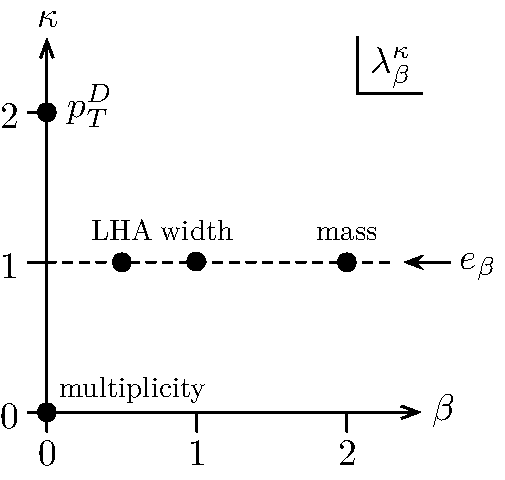
\includegraphics[scale = 0.7]{figures/lambda_space.pdf}
}
\caption{(a)  Two parameter family of generalized angularities, adapted from \cite{}.}
\end{figure}

A wide variety of quark/gluon discriminants have been proposed (see \cite{} for a catalog), but here we limit ourselves to a two-parameter family of generalized angularities \cite{}, shown in \Fig{fig:lambda_space}.  These are defined in general as
\begin{equation}
\label{eq:genang}
\genang{\kappa}{\beta} = \sum_{i \in \text{jet}} z_i^\kappa \theta_i^\beta,
\end{equation}
where $i$ runs over the jet constituents, $z_i$ is a momentum fraction, and $\theta_i$ is a (normalized) recoil-free angle. The parameters $\kappa$ and $\beta$ determine the energy and angle weighting, respectively.

For our $e^+ e^-$ study, we cluster jets using the $ee$-variant of the anti-$k_t$ algorithm \cite{}, with $|\vec{p}|$-ordered winner-take-all recombination \cite{} to determine the jet axis $\hat{n}$ (not the same as the jet momentum).  We then define
\be
z_i \equiv \frac{E_i}{E_{\rm jet}}, \qquad \theta_i \equiv \frac{\Omega_{i \hat{n}}}{R},
\ee
where $\Omega_{i \hat{n}}$ is the opening angle to the jet axis, and $R$ is the jet radius.  For our $pp$ study, we use the standard $pp$ version of anti-$k_t$, with $p_T$-ordered winner-take-all recombination, defining
\be
z_i \equiv \frac{p_{Ti}}{\sum_{j \in \text{jet}} p_{Tj}}, \qquad \theta_i \equiv \frac{R_{i \hat{n}}}{R},
\ee
where $R_{i \hat{n}}$ is the rapidity-azimuth distance to the jet axis.

By adjusting $\kappa$ and $\beta$, one can probe different aspects of the jet fragmentation.  We consider five benchmark values for $(\kappa, \beta)$:
\begin{align}
(0,0) &= \text{particle multiplicity},\\
(2,0) &\Rightarrow p_T^D \text{  \cite{} (specifically $\genang{2}{0} = (p_T^D)^2$)},\\
(1,0.5) & = \text{Les Houches Angularity (LHA)},\\
(1,1) &= \text{width},\\
(1,2) & \Rightarrow \text{mass} \text{ (specifically $\genang{1}{2} \simeq m_{\rm jet}^2 / p_{T{\rm jet}}$)}.
\end{align}
Except for the LHA, these angularities (or their close cousins) have already been used in quark/gluon studies.  The LHA has been included to have a angularity that weights energy more heavily than angle, similar in spirit to the $\beta = 0.2$ value advocated in \Ref{}.

With $\kappa = 1$, there is an alternative version of the angularities based on energy correlation functions \jdt{not sure about my definition here, especially factors of 2.}
\be
\text{ecf}_\beta = \frac{1}{2}\sum_{i \not= j \in \text{jet}} z_i z_j \theta_{ij}^\beta \simeq \genang{1}{\beta},
\ee
where equality holds in the extreme eikonal limit.  Amusingly, $\lim_{\beta \to 0} \text{ecf}_\beta = 1 - 2 \genang{2}{0}$ \cite{}.  To avoid a proliferation of curves, we will not show any results for $\text{ecf}_\beta$.  We will also neglect quark/gluon discriminants that take into account azimuthal asymmetries within the jet, such as elliptically and 2-subjettiness.

\subsection{Metrics for Discrimination Power}

Since we will be testing many Monte Carlo variants, we need a way to quantify quark/gluon separation power in a robust way that can easily be summarized in a single number.  For that purpose we use classifier separation \cite{}:
\be
\Delta =  \frac{1}{2} \int \df \lambda \, \frac{\bigl(p_q(\lambda) - p_g(\lambda)\bigr)^2}{p_q(\lambda) + p_g(\lambda)},
\ee
where $p_q$ ($p_g$) is the probability distribution for a quark-tagged (gluon-tagged) sample.  Here, $\Delta = 0$ corresponds to no discrimination power and $\Delta = 1$ corresponds to perfect discrimination power.

For ease of comparison to previous results, we will also show some results in terms of ROC curves.  At a point ($q$,$g$) on the ROC curve, where $q,g \in [0,1]$, one can define a selection that yields $q$ efficiency for quarks and $g$ mistag rate for gluons, or equivalently, a $(1-g)$ efficiency for gluons for a $(1-q)$ mistag rate for quarks.  From the ROC curve, we define five benchmark points, visualized in \Fig{fig:roc_curve}:  \jdt{Do we really want to show all of these?  I suspect not}
\begin{align}
\{ g^{\rm  rej}_{50} ,   g^{\rm  rej}_{20}\} : \quad & \text{Gluon rejection rate at \{50\%, 20\%\} quark efficiency}; \\
\{q^{\rm rej}_{50} ,  q^{\rm rej}_{20}\} : \quad & \text{Quark rejection rate at \{50\%, 20\%\} gluon efficiency}; \\
s^{\rm rej} : \quad & \text{Symmetric rejection rate at $s^{\rm rej}$ efficiency}.
\end{align}
For all of these measures, $x^{\rm rej} \in [\frac{1}{2},1]$, where $\frac{1}{2}$ corresponds to no discrimination and $1$ corresponds to optimal discrimination.  \jdt{This next sentence is no longer truth, I think.}  To assign statistical errors to these quantities in Monte Carlo, we make the simplifying assumption that the uncertainty is only due to Poisson statistics on the $x^{\rm rej}$ value.

\begin{figure}
\centering
\subfloat[]{
\label{fig:roc_curve}
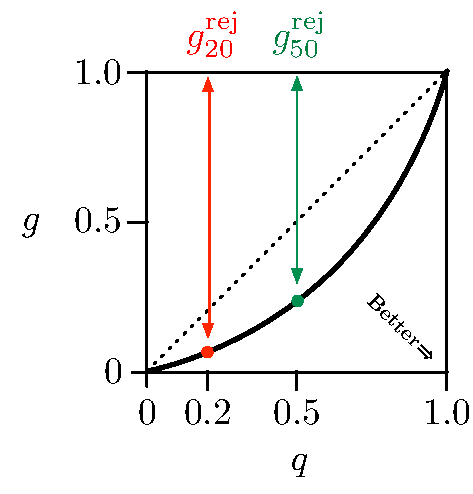
\includegraphics[scale = 0.85]{figures/roc_curve}
}
$\quad$
\subfloat[]{
\label{fig:truth_overlap}
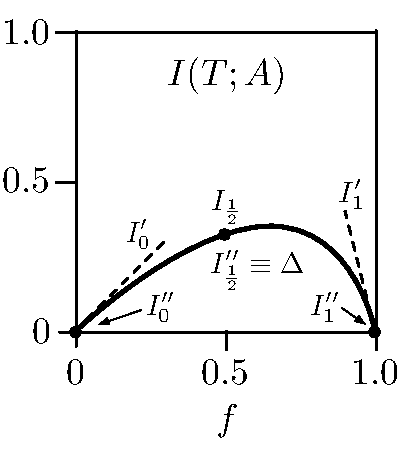
\includegraphics[scale = 0.85]{figures/truth_overlap}
}
\caption{(a) Five ROC Curve benchmark points.  (b) Six mutual information benchmark values.}
\end{figure}

\jdt{The discussion below should be simplified since we aren't going to show all of these anymore.}  An alternative way to quantify discrimination power is through mutual information, which counts the number of ``bits'' of information gained from measuring a discriminant variable (see \cite{Larkoski:2014pca}).  Given a sample with quark fraction $f \in [0,1]$ and gluon fraction $(1-f)$, the mutual information with the truth (a.k.a. the truth overlap) is:
\be
I(T;A) = \int \df a \left(f \, p_q(a) \log_2 \frac{p_q(a)}{p_{\rm tot}(a)} + (1-f) \, p_g(a) \log_2 \frac{p_g(a)}{p_{\rm tot}(a)}   \right),
\ee
where
\be
p_{\rm tot}(a) = f \, p_q(a) + (1-f) \, p_g(a).
\ee
The minimum value of $I(T;A)$ is $0$ (no discrimination) and the maximum value is
\be
I(T;A)_{\rm max} = f \log_2 \frac{1}{f} + (1-f) \log_2 \frac{1}{1-f},
\ee
which equals $1$ for $f = \frac{1}{2}$.

The choice $f = 1/2$ was used in \Ref{Larkoski:2014pca}, $I(T;A)\big|_{f = \frac{1}{2}} \equiv I_{\frac{1}{2}}$, though other $f$ choices are plausible.  The first derivative at $f = 1/2$ is not particularly enlightening, but the second derivative is related to classifier separation defined above
\be
- \frac{\log 2}{4} \frac{\partial^2 I(T;A)}{\partial f^2} \Big|_{f = \frac{1}{2}} \equiv I''_\frac{1}{2} \equiv \Delta
\ee
where the normalization has been set such that $I''_\frac{1}{2} \in [0,1]$.  At $f = 0$ and $f = 1$, the mutual information itself is zero, but the derivatives are related to other concepts in statistics:
\be
\frac{\partial I}{\partial f} \Big|_{f = 0} \equiv I'_0 = \int \df a \, p_q(a)  \log_2 \frac{p_q(a)}{p_g(a)}, \qquad - \log 2 \,  \frac{\partial^2 I}{\partial f^2} \Big|_{f = 0} \equiv I''_0 = \int \df a \,  \frac{p_q(a)^2}{p_g(a)},
\ee
\be
- \frac{\partial I}{\partial f} \Big|_{f = 1} \equiv I'_1 = \int \df a \, p_g(a) \log_2 \frac{p_g(a)}{p_q(a)}, \qquad - \log 2 \, \frac{\partial^2 I}{\partial f^2} \Big|_{f = 1} \equiv I''_1 = \int \df a \, \frac{p_g(a)^2}{p_q(a)}.
\ee
The first derivative is sometimes called relative entropy and the second derivative is sometimes called discrimination significance.  However, all of these quantities become singular if the probability distribution is zero, so we will only quote the values at $f = \frac{1}{2}$, visualized in \Fig{fig:truth_overlap}:
\be
\{I_\frac{1}{2}, I''_{\frac{1}{2}} \}.
\ee
To assign statistical errors to these quantities in Monte Carlo, we evaluate $I(T;A)$ in bins of $a$ and use Poisson statistics.  Note that there is a binning bias in $I_\frac{1}{2}$, so we use the method explained in Appendix A.3 of \Ref{Larkoski:2014pca} and use half the $\Delta a$ bin size on the combined quark/gluon sample compared to the individual quark/gluon samples.

\subsection{Parton-level Quark/Gluon Tags}

\jdt{Do we want to say anything here about QCDAware or flavored jet algorithms?  Are we going to use them?}

\section{Idealized Quark/Gluon Tagging}
\label{sec:ee}

\jdt{Start with hadron-level, since that is easiest to explain, then do parton level to explore further.}

\subsection{Hadron-Level Performance}

\begin{figure}
\centering
\subfloat[]{
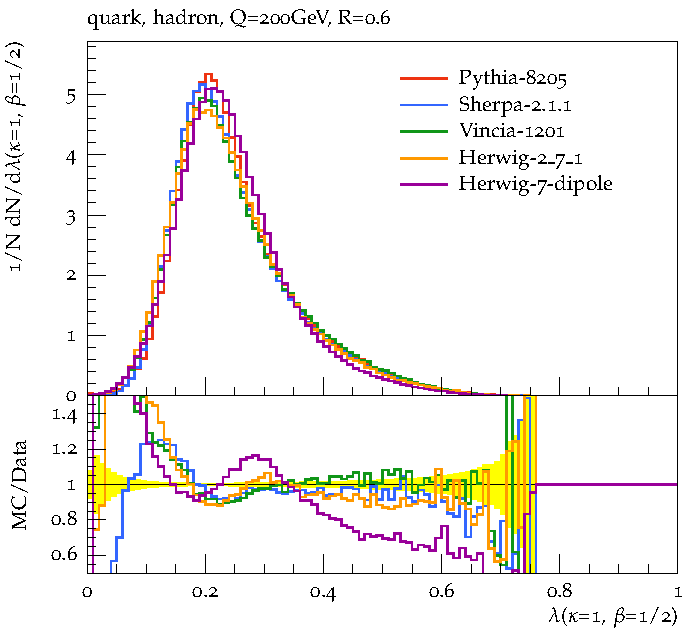
\includegraphics[width = 0.45\columnwidth]{figures/GA_10_05_R6_hadron_quark.pdf}
\label{fig:LHA_hadron_quark}
}
$\quad$
\subfloat[]{
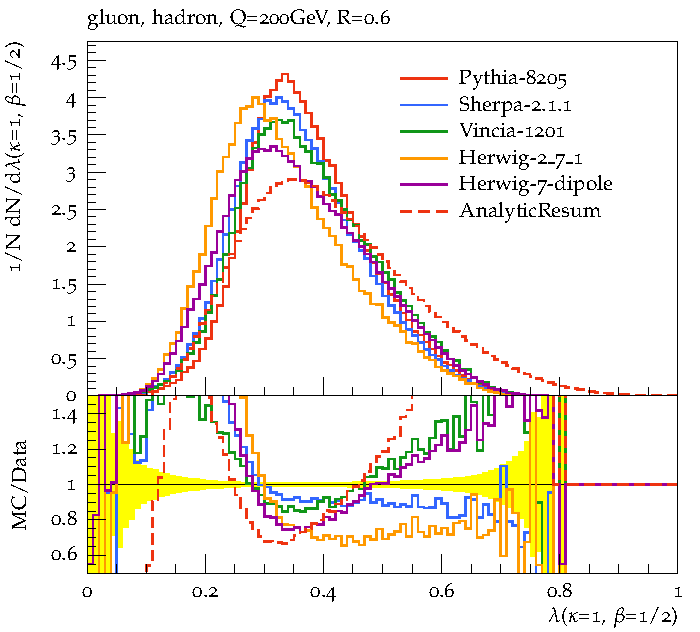
\includegraphics[width = 0.45\columnwidth]{figures/GA_10_05_R6_hadron_gluon.pdf}
\label{fig:LHA_hadron_gluon}
}
$\quad$
\subfloat[]{
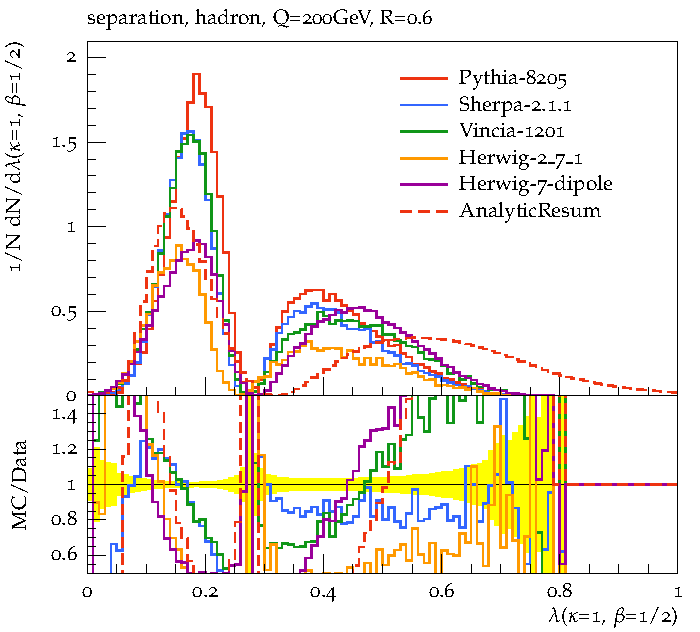
\includegraphics[width = 0.45\columnwidth]{figures/GA_10_05_R6_hadron_separation.pdf}
\label{fig:LHA_hadron_separation}
}
\caption{hadron-level (a) quark (b) gluon (c) separation}
\end{figure}

\begin{figure}
\centering
\subfloat[]{
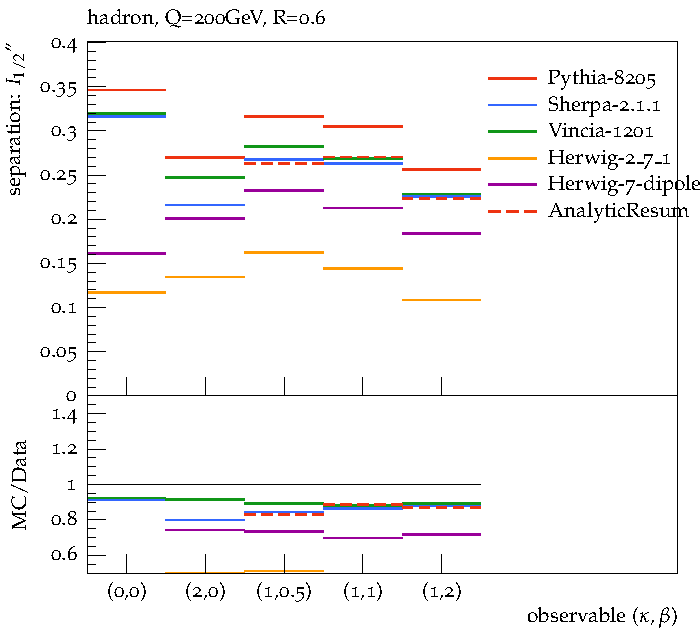
\includegraphics[width = 0.45\columnwidth]{figures/I2_R6_hadron__all.pdf}
\label{fig:summary_hadron_all}
}
\caption{(a) all comparison}
\end{figure}

\begin{figure}
\centering
\subfloat[]{
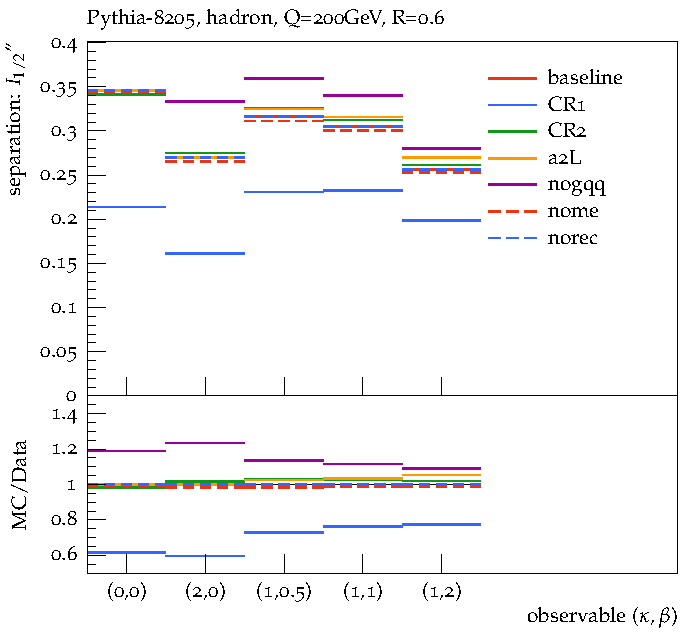
\includegraphics[width = 0.45\columnwidth]{figures/I2_R6_hadron_pythia.pdf}
\label{fig:summary_hadron_pythia}
}
$\quad$
\subfloat[]{
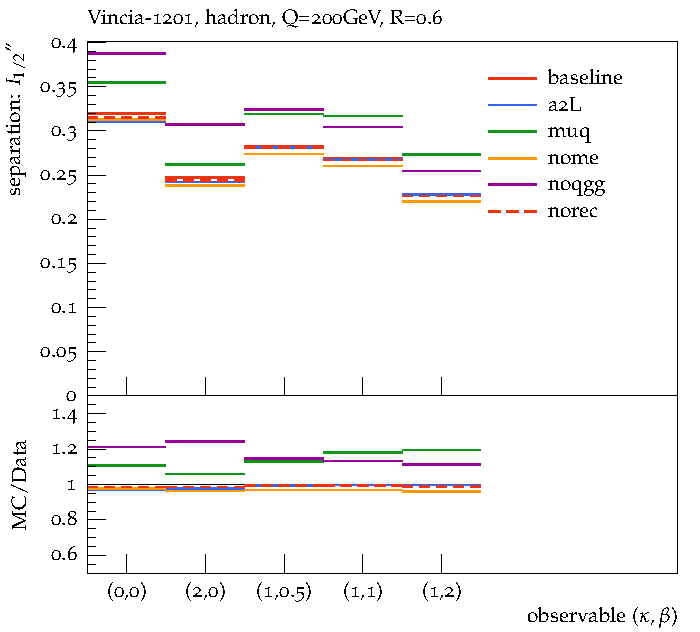
\includegraphics[width = 0.45\columnwidth]{figures/I2_R6_hadron_vincia.pdf}
\label{fig:summary_hadron_vincia}
}
$\quad$
\subfloat[]{
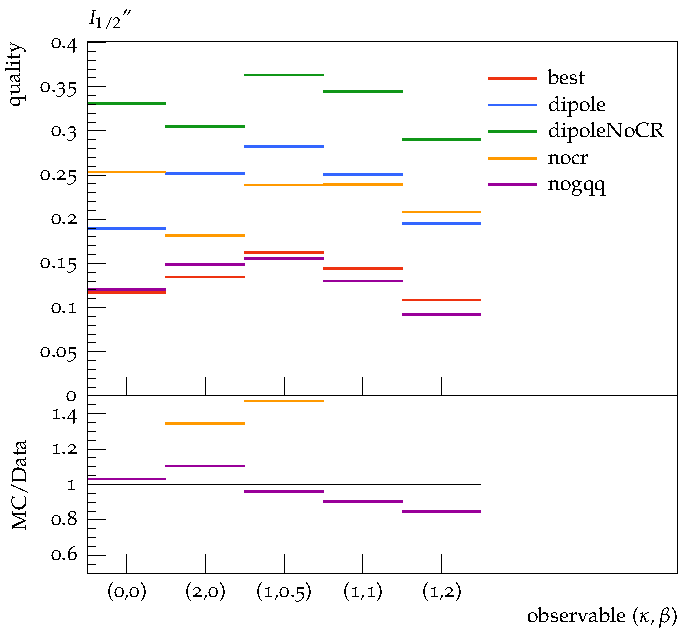
\includegraphics[width = 0.45\columnwidth]{figures/I2_R6_hadron_herwig.pdf}
\label{fig:summary_hadron_herwig}
}
$\quad$
\subfloat[]{
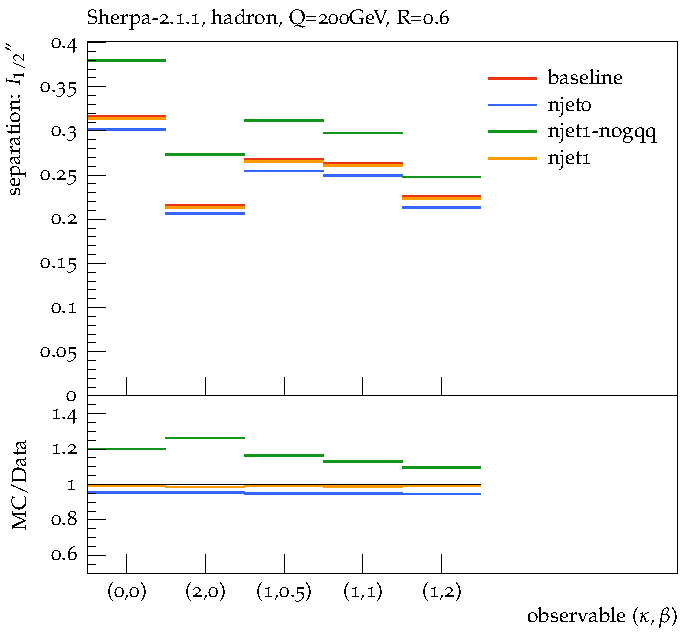
\includegraphics[width = 0.45\columnwidth]{figures/I2_R6_hadron_sherpa.pdf}
\label{fig:summary_hadron_sherpa}
}
\caption{variants on (a) pythia (b) vincia (c) herwig (d) sherpa}
\end{figure}


\begin{figure}
\centering
\subfloat[]{
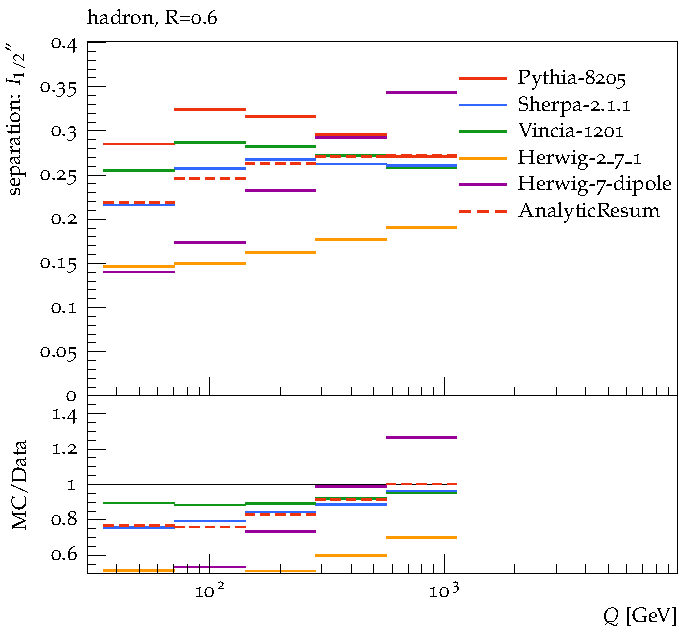
\includegraphics[width = 0.45\columnwidth]{figures/I2_GA_10_05_hadron_Qdep.pdf}
\label{fig:sweep_Q_hadron}
}
$\quad$
\subfloat[]{
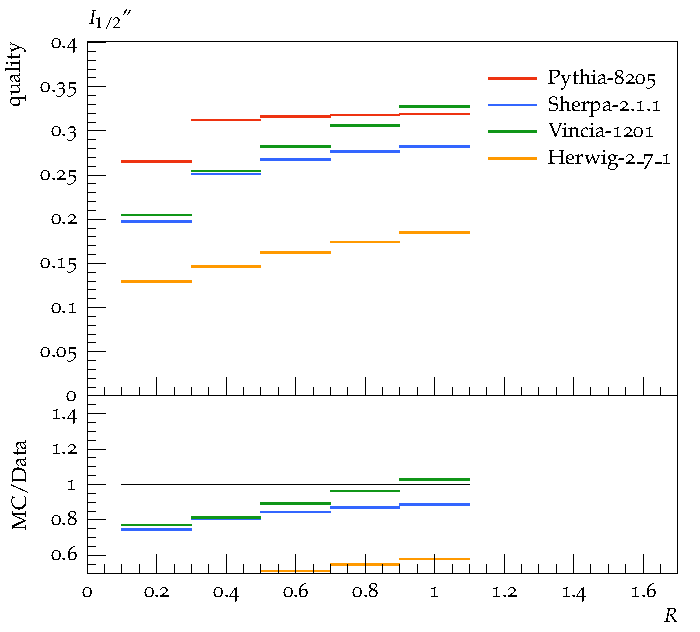
\includegraphics[width = 0.45\columnwidth]{figures/I2_GA_10_05_hadron_Rdep.pdf}
\label{fig:sweep_R_hadron}
}
$\quad$
\subfloat[]{
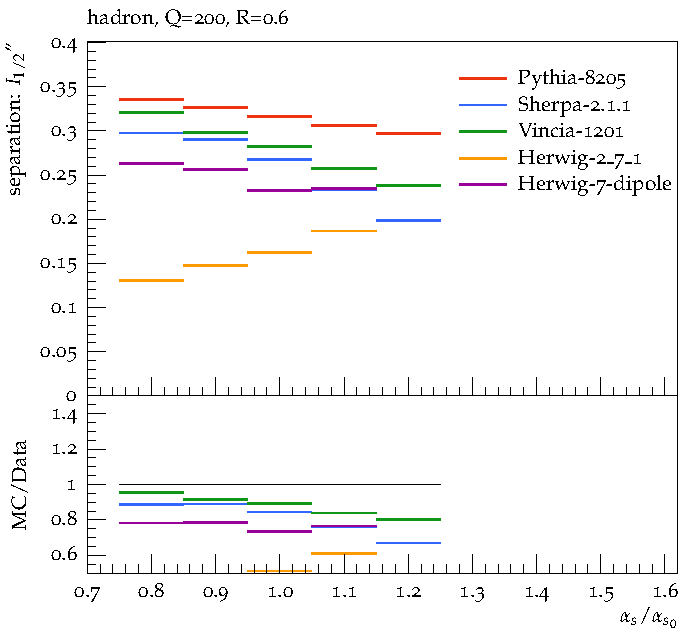
\includegraphics[width = 0.45\columnwidth]{figures/I2_GA_10_05_hadron_alphadep.pdf}
\label{fig:sweep_as_hadron}
}
\caption{Hadron-level (a) $Q$ (b) $R$ (c) $\alpha_s$}
\end{figure}


\subsection{Parton-Level Performance}


\begin{figure}
\centering
\subfloat[]{
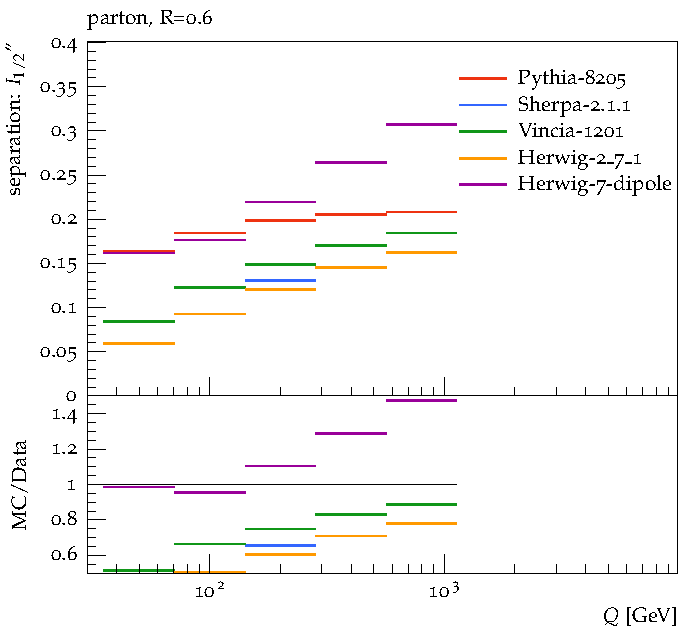
\includegraphics[width = 0.45\columnwidth]{figures/I2_GA_10_05_parton_Qdep.pdf}
\label{fig:sweep_Q_parton}
}
$\quad$
\subfloat[]{
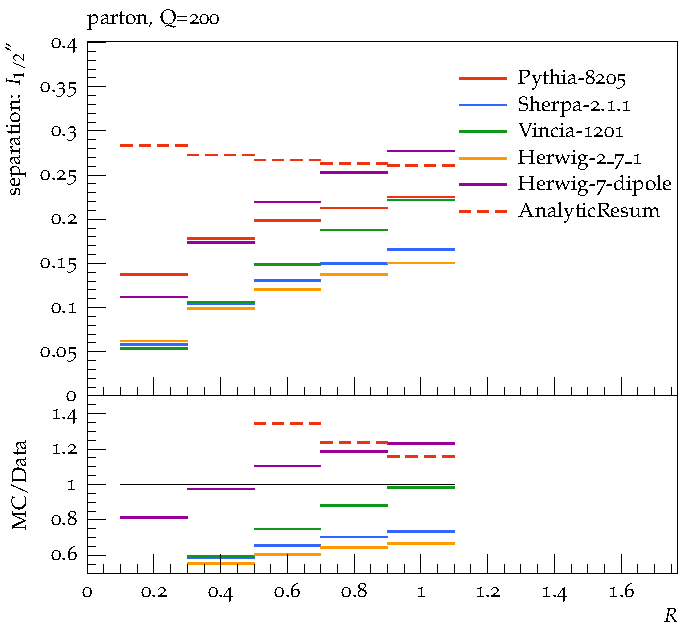
\includegraphics[width = 0.45\columnwidth]{figures/I2_GA_10_05_parton_Rdep.pdf}
\label{fig:sweep_R_parton}
}
$\quad$
\subfloat[]{
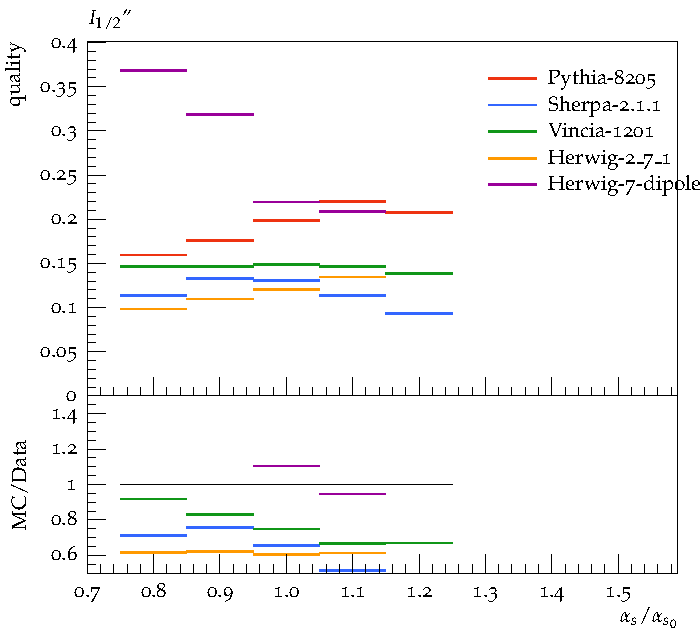
\includegraphics[width = 0.45\columnwidth]{figures/I2_GA_10_05_parton_alphadep.pdf}
\label{fig:sweep_as_parton}
}
\caption{Parton-level (a) $Q$ (b) $R$ (c) $\alpha_s$}
\end{figure}







\subsection{Predictions from Resummation}

\jdt{Talk to Frank if this is feasible.}

\section{Quark/Gluon Tagging at the LHC}
\label{sec:pp}

\subsection{Enriched Quark/Gluon Samples}

\subsection{Tagging Performance}


\section{Conclusions}
\label{sec:conclude}




\begin{acknowledgments}
We thank Jon Butterworth, Peter Loch, Alexander Schmidt \jdt{and anyone else who wants to take their name off of the paper}.

\end{acknowledgments}


\bibliographystyle{JHEP}
\bibliography{lh2015_qg}

\end{document}
